\chapter{Angle Measurement with Build-in Sensors}\label{chap:CompFilter} \fxnote{different chapter names, since this might be more of a chapter how to get IMU working than just about complementary filter?, B}
It is a goal to get the Cubli setup to balance the frame in an upright position independently of the baseplate orientation.

As described in \secref{sec:Sensors} there are two IMUs mounted on the frame of the Cubli. They can be used to achieve this goal since they only depend on the absolute angle and they can also be used in the full Cubli.

\section{Angle Calculations from the IMUs}
The angular position of the Cubli can be calculated using the accelerometer, the gyroscope or combining both. In this section each of the options is describe and analyzed.

\subsection{Angle from the Accelerometer}
To determine the angle of the frame with the accelerometer it is needed to get the measurements from two of the three axes. The two measurements needed are the ones in line with the frames movement direction, based on the way the IMU is mounted, as shown in \ref{accelerometer}.
\begin{figure}[H]
	\centering
	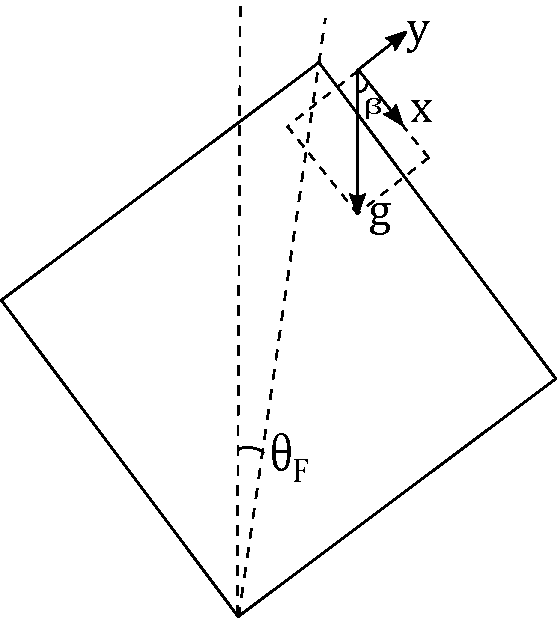
\includegraphics[scale=0.5]{figures/accelerometer}
	\caption{Position of the IMU in the setup}
	\label{accelerometer}
\end{figure}\vspace{-5mm}

As shown in the figure the angle can be found using \eqref{accelAngle}.
%
\begin{flalign}
	\eq{accel\_\theta_{F}} {\arctan\left(\frac{y}{x}\right) + 0.84}
	\label{accelAngle}
\end{flalign}

Based on the data from \appref{app:IMUMeasurementsAppendix}, a calculation of the angle can be done, whose result is shown in \figref{angleAcc}.
%
\begin{figure}[H]
	\centering
	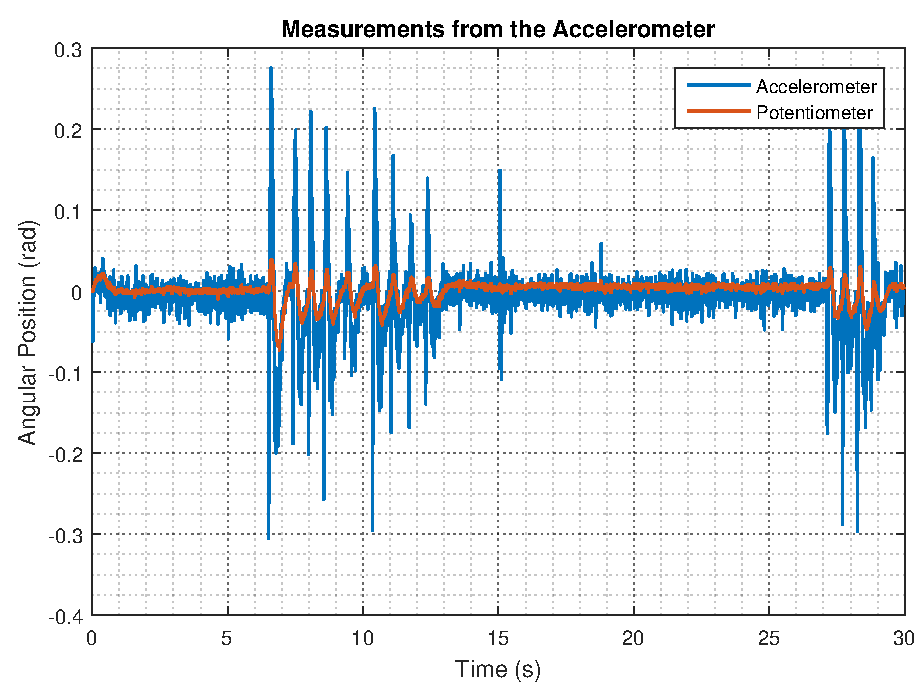
\includegraphics[scale=0.65]{figures/angleAcc}
	\caption{Angular position calculation with the data of the accelerometer}
	\label{angleAcc}
\end{figure}\vspace{-5mm}
%
 It can be seen that the accelerometer can detect changes in the angle, but has problems with noise and measuring fast changes in the angle.\fxnote{source?, also reason for error seems to be fast and large?} 

\subsection{Angle from the Gyroscope}
The angle of the frame can be found with the gyroscope by integrating the angular velocity measured by the gyroscope on the axis aligned with the direction of motion of the frame as shown in \ref{systemDescription}. \fxnote{correct the ref to the picture of the cubli setup}
\begin{flalign}
	\eq{gyro\_\theta_{F}} {\int \omega_{F}}
	\label{accelGyro}
\end{flalign}
The problem with the data from the gyro is an accumulating error which is caused by the integration done to convert angular velocity into an usable angle. It is also known that the gyros will exhibit a drifting error when experiencing small and slow movement.\fxnote{source on gyro error?, B}

\subsection{Data fusing} \fxnote{better section name?}
To counteract the drift of the gyroscope and the errors of the accelerometer a complementary filter can be used to combine both measurements from the two IMUs mounted on the Cubli frame.\fxnote{elaborate on the errors} 

The two angle measurements of the IMU are sent through a filter and then summed in order to get an angle of the Cubli's frame.

\begin{figure}[H]
	\begin{tikzpicture}[ auto,
thick,                         %<--setting line style
node distance=2cm,             %<--setting default node distance
scale=1.5,                     %<--|these two scale the whole thing
every node/.style={scale=1.5}, %<  |(always change both)
>=triangle 45 ]                %<--sets the arrowtype
\draw%--------------------------------------------------------------------------------------------

node[shape=coordinate][](acc) at (0,0){acc}			% start of acc signal path

node(lowpas) at (6,0) [block] {\Large $\ \frac{1}{\tau \cdot s + 1}$ }

node[shape=coordinate][](gyro) at (0,-2){}		% start of gyro signal path

node(integrate) at (3,-2) [block] {\Large $\frac{1}{s}$}

node(highpas) at (6,-2) [block] {\Large $\ \frac{\tau \cdot s}{\tau \cdot s + 1}$ }

node(sum) at (8,-1) [sum] {$\sum$}


node[shape=coordinate][](angle) at (10,-1){}		% output of the complementary filter
;

\draw[->](acc) -- node {accel$\_\theta_{F}$} (lowpas);
\draw[->](gyro) -- node {gyro$\_\omega_{F}$} (integrate);
\draw[->](integrate) -- node {} (highpas);

\draw[->](highpas) -| node {} (sum);
\draw[->](lowpas) -| node {} (sum);


\draw[->](sum) -- node {$\theta_{F}$} (angle);

\end{tikzpicture}

	\centering
	\caption{Block diagram of the complementary filter setup used with the IMU on the Cubli}
	\label{blockDrawingComplementaryFilter}
\end{figure}

The filter for the IMU is designed as shown in \figref{blockDrawingComplementaryFilter} with a low pass filter on the measurements from the accelerometer, and an integration followed by a high pass filter on the measurements from the gyroscope. \cite{OlliW} \fxnote{might not be the correct source for this part, but it is a source that is useful for the part, B}
\begin{flalign}
	\eq{\theta_{F}} {\frac{1}{ 1 + \tau \cdot s} \cdot accel\_\theta_{F}}   &\\
	\eq{\theta_{F}} {\frac{\tau \cdot s}{ 1 + \tau \cdot s} \cdot \frac{1}{s} \cdot gyro\_\dot{\theta}_{F}}&
	\label{complementaryBlockFilters}
\end{flalign}
Combining the two equations yields \eqref{complementaryCombinedFilter}
\begin{flalign}
	\eq{\theta_{F}} {\frac{1}{ 1 + \tau \cdot s} \cdot accel\_\theta_{F} + \frac{\tau \cdot s}{ 1 + \tau \cdot s} \cdot \frac{1}{s} \cdot gyro\_\dot{\theta}_{F} = \frac{accel\_\theta_{F} + \tau \cdot gyro\_\dot{\theta}_{F}}{1 + \tau \cdot s}} &
	\label{complementaryCombinedFilter}
\end{flalign}
The \si{\tau} is the cut-off frequency of the two filters. Changing this constant decides how much the two different sensor measurements weight in on the combined angle.
 
\section{Discretization of the Complementary Filter} 
In oder to use the complementary filter on the cubli it needs to be discretized. This is done with the bilinear transformation method where \si{s = \frac{2}{\Delta T}\cdot \frac{1 - z^{-1}}{1 + z^{-1}}}, with a sample time of 
Rewritting \eqref{complementaryCombinedFilter} yields
\begin{flalign}
 	\eq{\theta_{F}} {\frac{1}{1 + \tau \cdot s} \cdot (accel\_\theta_{F} + \tau \cdot gyro\_\dot{\theta}_{F})} &
 	\label{discreteComplementaryFilter1}
\end{flalign}
Now s is replaced
\begin{flalign}
  	\eq{\theta_{F}} {\frac{1}{1 + \tau \cdot \frac{2}{\Delta T}\cdot \frac{1 - z^{-1}}{1 + z^{-1}}} \cdot (accel\_\theta_{F} + \tau \cdot gyro\_\dot{\theta}_{F})} &
  	\label{discreteComplementaryFilter2}
\end{flalign}
%
%\begin{flalign}
%  	\eq{\Updownarrow \theta_{F}} {\frac{\Delta T \cdot (1 + z^{-1})}{\Delta T \cdot (1 + z^{-1})+2\cdot (1 - z^{-1})\cdot \tau} \cdot (accel\_\theta_{F} + \tau \cdot gyro\_\dot{\theta}_{F})}
%  	\label{discreteComplementaryFilter3}
%\end{flalign}
  %
\begin{flalign}
   	\eq{\Updownarrow \theta_{F}} {\frac{\Delta T + \Delta T \cdot z^{-1}}{(2\cdot \tau + \Delta T) - (2\tau - \Delta T)\cdot z^{-1}} \cdot (accel\_\theta_{F} + \tau \cdot gyro\_\dot{\theta}_{F})} &
\end{flalign}\label{discreteComplementaryFilter4}
%
\begin{flalign}
	\eq{\Updownarrow \theta_{F} \cdot ((2\cdot \tau + \Delta T) - (2\tau - \Delta T)\cdot z^{-1})} {\Delta T + \Delta T \cdot z^{-1} \cdot (accel\_\theta_{F} + \tau \cdot gyro\_\dot{\theta}_{F})} &
\end{flalign}\label{discreteComplementaryFilter5}
%
\begin{flalign}
	\eqOne{\Updownarrow \theta_{F}[n] \cdot (2\cdot \tau + \Delta T) - \theta_{F}[n-1] \cdot (2\tau - \Delta T)} {\Delta T \cdot (accel\_\theta_{F}[n] + accel\_\theta_{F}[n-1]} 
	\eqTwo{ + \tau \cdot gyro\_\dot{\theta}_{F}[n] + \tau \cdot gyro\_\dot{\theta}_{F}[n+1])} 
\end{flalign}	\label{discreteComplementaryFilter6}
%  
\begin{flalign}
	\eqOne{\Updownarrow \theta_{F}[n]}{\frac{(2\cdot \tau + \Delta T)}{2\cdot \tau + \Delta } \cdot \theta_{F}[n-1] + \frac{\Delta T}{2\cdot \tau + \Delta T} \cdot accel\_\theta_{F}[n] + \frac{\Delta T}{2\cdot \tau + \Delta T} \cdot accel\_\theta_{F}[n-1]} 
	\eqTwo{ + \frac{\Delta T \cdot \tau}{2\cdot \tau + \Delta T} \cdot gyro\_\dot{\theta}_{F}[n] + \frac{\Delta T \cdot \tau}{2\cdot \tau + \Delta T} \cdot gyro\_\dot{\theta}_{F}[n-1]} 
\end{flalign} 	\label{discreteComplementaryFilterFinal}
%
Implementing \eqref{discreteComplementaryFilterFinal} yields to following piece of code. \fxnote{USE the current form in the controller code file}
%
\begin{lstlisting}[caption  = {Code for the implementation of the complementary filter in C++},
label    = codeCompFilter ]
/**
*  delta_T is the sampling time = 0.01 s
*  tau is the cut-off frequency of the low and high pass filters
*/
theta_f[n] = ((2*tau-delta_T) / (2*tau+delta_T)) * theta[n-1] + 
	(delta_T / (2*tau+delta_T)) * (acc_theta[n] + tau * gyro_thetaDot[n] + 
	acc_theta[n-1] + tau * gyro_thetaDot[n-1]) 
\end{lstlisting}

\section{Calculation of the Cut-off Frequency}
The cut-off frequency for the filters can be determined by using SensTool and the data obtained through the test detailed in \appref{app:IMUMeasurementsAppendix}. 

The toolbox uses the data form the potentiometer as the real output of the system, the data from the IMUs as the input and the modeling of the system is done through \eqref{discreteComplementaryFilterFinal}. With this data it can find the optimal value for \si{\tau} based on the difference between the angle measured by the potentiometer and an angle calculated from accelerometer and gyroscope measurements done during the same test.

The final fit can be seen in \figref{filterSensTool} and it gives an optimal \si{\tau\ =\ 0,5399\ s}. This results in a cutting frequency for the filter equal to \si{11,63\ rad \cdot s^{-1}}.
%
\begin{figure}[H]
	\centering
	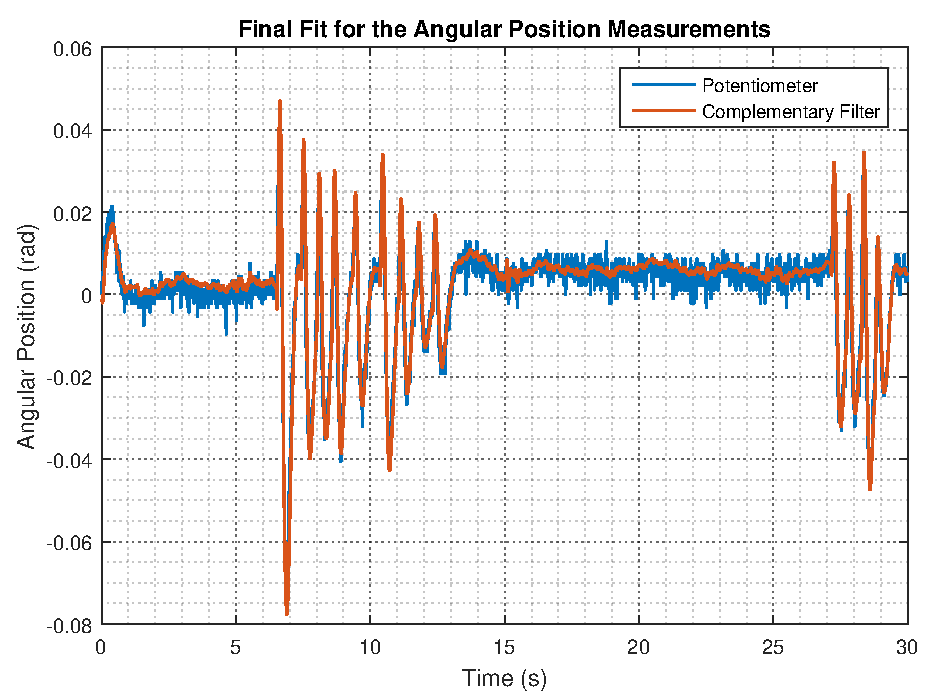
\includegraphics[scale=0.65]{figures/filterSensTool}
	\caption{Final result od the complementary filter compared with the data from the potentiometer}
	\label{filterSensTool}
\end{figure}\vspace{-5mm}
%